\section{Future Research }
Our main goal is to develop a tool for extracting structural information from a cryoEM map at various resolutions.
Specifically, given a cryoEM map of an assembly, we intend to localize regions in the map of known and important atomic structure.
Such regions are called anchors.
The structure of the anchors will depend on the map resolution.
For very high-resolution maps (3 Angstroms and better) amino acids and aromatic rings will be identified. 
For intermediate  resolution maps (4- 6 Angstroms and better)  binding sites and protein-protein interfaces will be identified.

The general strategy will be to train a classification Convolution Neural Network (CNN) for each anchor type. Given a small cube of cryoEM  density a  classification CNN  will assign a label to the cube. 
Cubes where an atomic structure was identified with high confidence will be labelled as anchors.  The whole map will be searched for anchors by transforming a classification CNN into a Full Convolutional Network (FCN).
\subsection{Detecting Amino Acids in very high resolution maps.}\label{s:aa_task}
We should continue to develop the techique of Amino Acid detection in High Resolution Maps.
Given an electron density map of a protein/macromolecular assembly, our task is to detect voxels in this map, which correspond to the location of the centres of mass of specific amino acids.
The goal is to report only those amino acids, which have been detected with high confidence, nicknamed "anchors".
The detection procedure consists of  extracting small cubes from a map and applying  a \textit{selective classifier}  to each cube.
\paragraph{Selective Classification}. A selective classification is a classification with a reject option. A \textit{selective classifier} is a pair of functions $f(x)$, called the \textit{classifier}, and $g(x)$ is  called \textit{selection  function}. The classification of a proposal $x$ is as follows:
\begin{equation}
(f,g)(x) = \left\{ \begin{array}{lcl}
f(x) & if & g(x) = 1 \\
NONE & if & g(x) = 0 \\
\end{array}
\right.
\end{equation}

We anticipate that integrating sythetic and X-ray crystallography data will result in  improvement of  the performance of our algorithm.

\subsubsection{Training Phase}
In a training process the parameters of a selective classification are adjusted by running backpropagation algorithm on a large amount of labeled data. 
The main limitation of the training phase is small amount of high resolution cryo EM maps.
There are two additional data sources which we try to use in the training phase:
\begin{enumerate}
    \item Crystallographic data. PDBe database \cite{Velankar2012} contains tens of thousands of electron density maps.
    \item Synthetic Data i.e., cryo-EM maps obtained by simulation program from a given atomic structure.  
\end{enumerate}
Both sources mentioned above suffer from the \textbf{domain shift}, i.e., the difference in the data distribution between train and test sets. 
To address this issue, two \textbf{domain adaptation} approaches are proposed to bridge the gap between the source and target domains: utilizing crystallography data (Section ~\ref{s:fut_xray}) and semi-supervised approach (Section ~\ref{s:fut_semi_super}) .


\subsubsection{Utilizing X-ray Crystallography Data }\label{s:fut_xray}
We suggest to use the Domain Confusion architecture presented in \cite{Hoffman2017}, see Fig. \ref{f:dom_conf_1}.
Up to  date for most of the molecular   complexes in cryo-EM dataset  X-ray data can be found for the same molecule or its close homolog.
Meaning that a one-to-one correspondence is available for entries in the target and source domain.
We will adjust the domain confusion network to take an advantage of the above fact by adding a new loss function member.

\subsection{Semi-Supervised Deep Learning Approach for Anchors Detection }\label{s:fut_semi_super} 
Semi-Supervised Deep Learning Approach presented at Fig ~\ref{f:semi_super} utilizes realistic cryo-EM map simulation for Anchors detection.
The query protein sequence is used to detect atomic models of structural homologs. 
This can be done by employing local alignment search tools (BLAST, PSI-PLAST, HHPred) or retrieving known structures from the protein family according to existing hierarchical classifications (SCOP \cite{Hubbard1999}, CATH \cite{Orengo1997}).
Retrieved homolog structures are fed to  the VAE-GAN simulation to create realistic cryo-EM maps (see Section  ~\ref{s:fut_gan} for details).
Created synthetic cryo-EM maps together with atomic models are used for fine tuning of the pretrained neural network. 
Anchors locations are obtained by running a fine-tuned network on the query map.
The presented approach has a number of advantages:
\begin{itemize}
    \item Sequence information is utilized in the anchor location task.
    \item Using homolog structures ensures that the training dataset and the query map have similar feature distributions.
    \item Training datasets of arbitrary size can be created.
\end{itemize}

\subsection{Annotating Secondary Structure in a Medium Resolution ($4 -6${\AA} ) cryo-EM maps}
The task is to assign each voxel in the qiven cryo-EM map to one of the three secondary structures: helix, beta-strand, coil.
This task is known as \textbf{semantic segmentation}.
The voxel is classified according to the cube in  the 3D map which surounds it.
Classification CNN converted to   Fully Convolutional Network  (FCN) is used.
The classification CNN is pretrained on a set of experimental cryo-EM maps  of medium resolution.
Fine tunnig achieved by training the last two layers on simulated data set as shown on Fig.~\ref{f:semi_super} and Section~\ref{s:fut_semi_super}




\begin{figure}
  \centering
	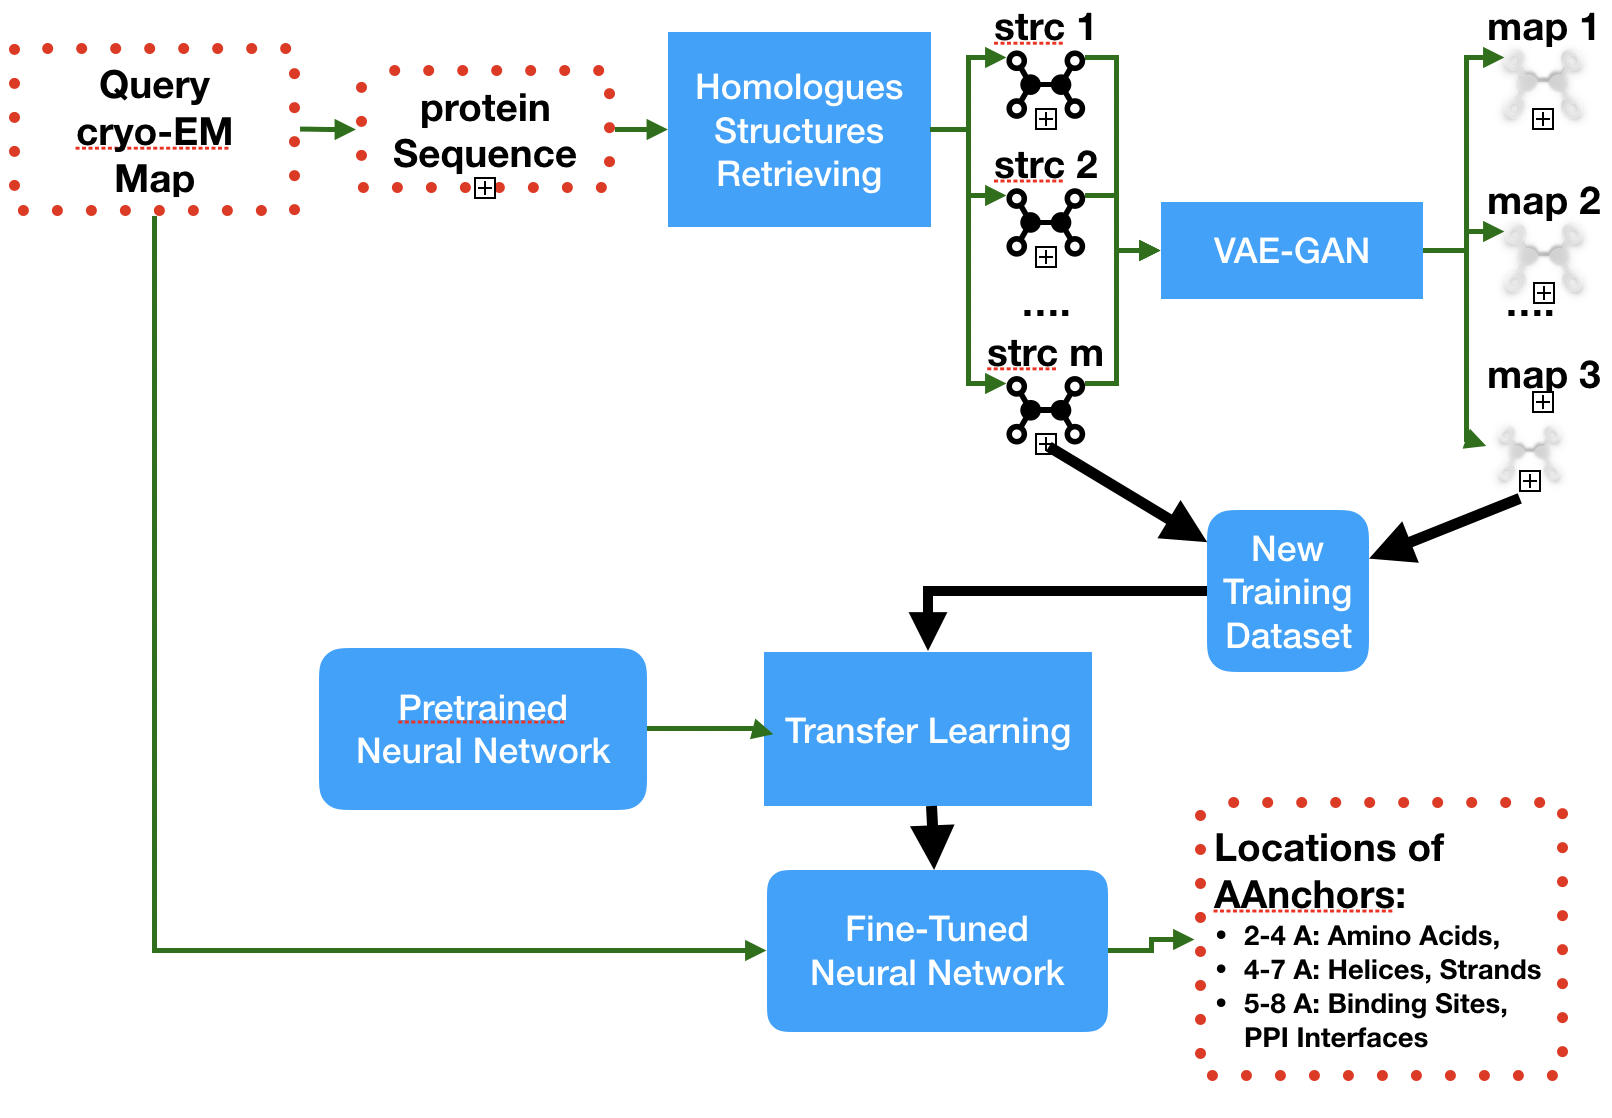
\includegraphics[scale=0.4]{picsnew/semi_super.png}
  \caption{Semi Supervised ML Algorithm for Locating Anchors}\label{f:semi_super}
\end{figure}



\subsection{Locating  Binding Sites in medium resolution cryo-EM maps }\label{bs_task}
Proteins with similar function often have active sites which are structurally similar. 
Active site structures  are usually conserved during evolution.
Despite the above facts, locating an active site for an unknown functionality is a challenging task.
This is due to the wide structual diversity of protein active sites.
Their  structural diversity can be reduced by existing sequence analysis algorithms. 
We propose a  four -phased algorithm for integrative location of binding sites - Fig.\ref{f:det_scheme4}.

In the \textbf{sequence analysis} phase possible reqions of binding sites are located in the query protein sequence.
This  can be done using traditional tools for finding conserved regions (conSurf \cite{Ashkenazy2010}  and others  \cite{Capra2007},  \cite{Fischer2008},  \cite{Rausell2010},  \cite{Lopez2011} ) or new Deep Learning Tools  (DeepBind \cite{Alipanahi2015}, and others \cite{Cui2019},  \cite{Chen2011ATPsiteResidues}).
Atomic models are created from the located sequence regions using existing modelling tools (Modeller , Rosetta).
In the \textbf{simulation} phase generated atomic models
are fed to VAE-GAN to create realistic synthetic cryo-EM maps of  expected binding  sites.
In the \textbf{transfer learning phase}  a pretrained CNN is fited to the new dataset, which consists of generated atomic models and synthetic cryo-EM maps.
Finally, in the \textbf{search} phase, the query map is fed to the fine-tuned neural network. 

\subsection{Calibration}
 In the anchor detection tasks( amino acids detection  Section \ref{s:aa_task} and binding site detection Section \ref{bs_task}) the confidence of reported detections matters.
 The goal is to filter out picks with confidence below a predefined threshold (say $80 \%$).
 This can be done by \textbf{calibration} of a detection network, using post-training methods such as \textbf{temperature scaling} \cite{Guo2017}.
 Another approach is to estimate the uncertainty of the neural network prediction by its training history \cite{Geifman2018}.
 
\subsection{Realistic cryo EM  Simulation : Generative Adversarial Network}\label{s:fut_gan}
Realistic cryo EM map simulation is the core of the algorithm presented above.
In the preliminary work we have developed cryo-GAN (Section \ref{s:c-GAN}).
The simulation uses Variational AutoEncoder (VAE) architecture combined with Generative Adversarial Network (GAN) to create  a cryo-EM map of an atomic structure.
While the preliminary results show that cryo-GAN is able to generate realistic cryo-EM maps, additional performance evaluation is required.
Moreover, we plan futher develop the simulation to make it a useful tool for algorithm developers working with cryo electron microscopy.


\begin{figure}
  \centering
	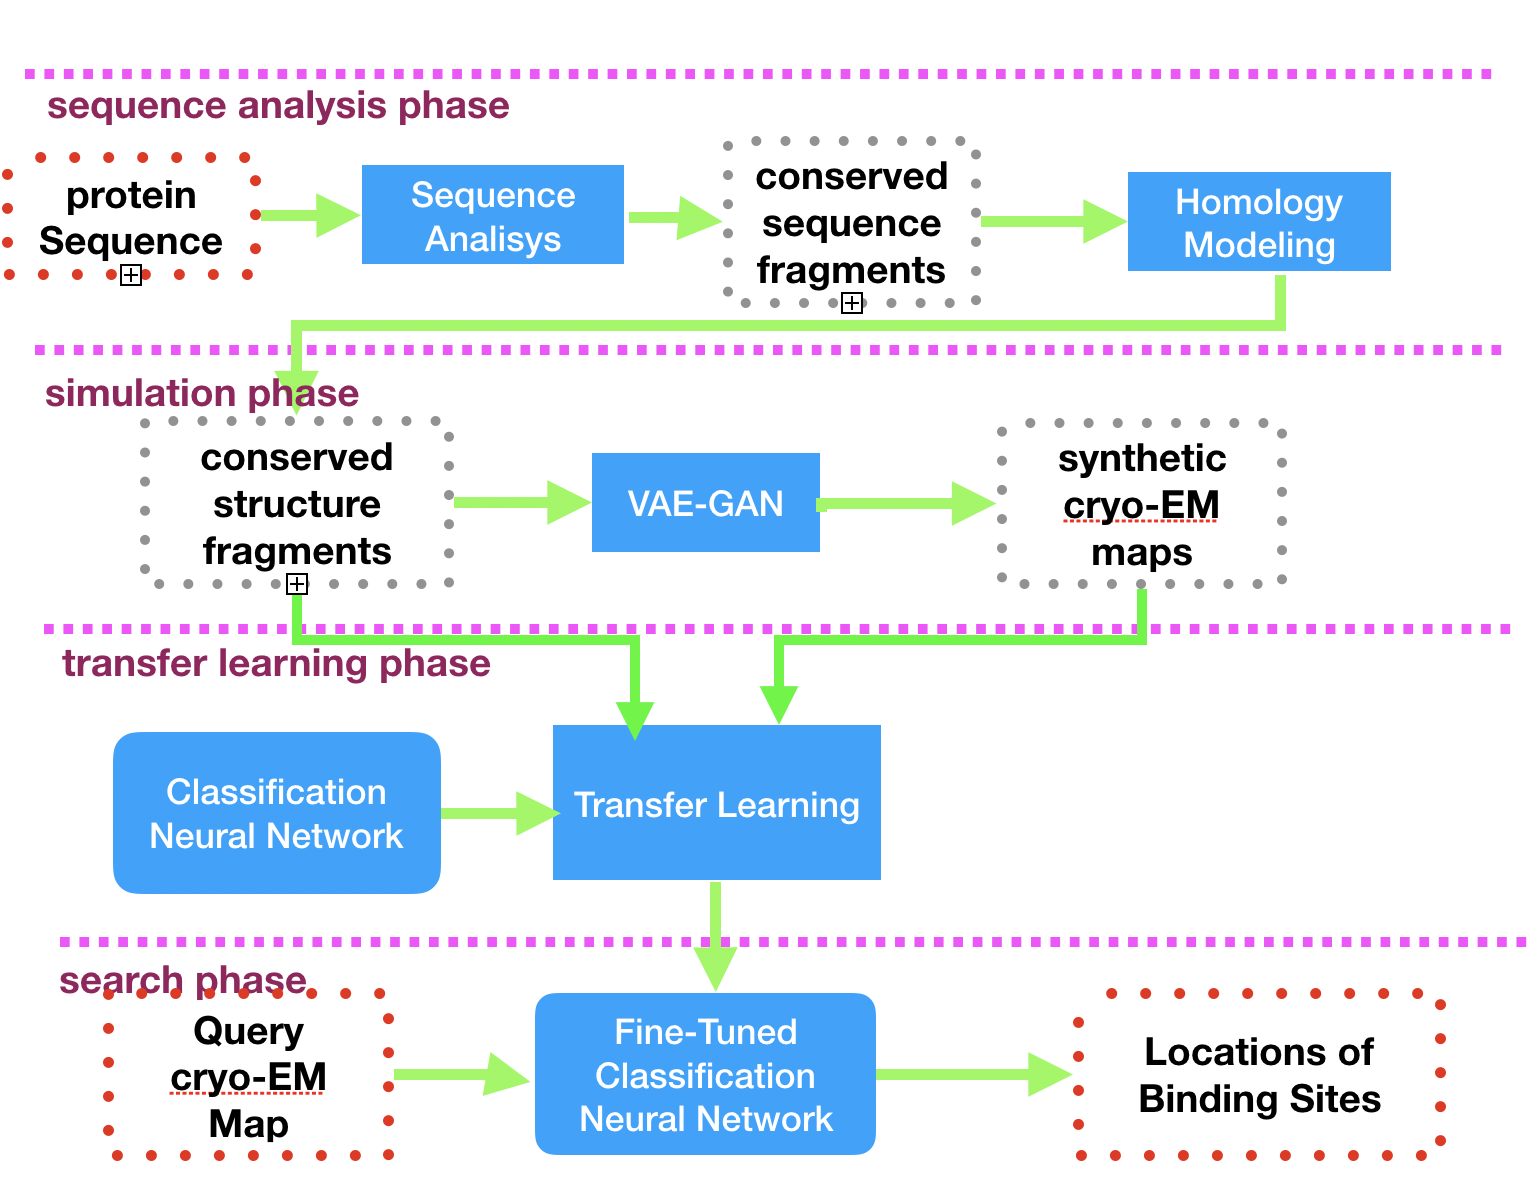
\includegraphics[scale=0.4]{picsnew/sch4.png}
  \caption{Finding Conserved Structures}\label{f:det_scheme4}
\end{figure}
